% Don't touch this %%%%%%%%%%%%%%%%%%%%%%%%%%%%%%%%%%%%%%%%%%%
\documentclass[11pt]{article}
\usepackage{fullpage}
\usepackage[left=1in,top=1in,right=1in,bottom=1in,headheight=3ex,headsep=3ex]{geometry}
\usepackage{graphicx}
\usepackage{float}
\usepackage{xcolor}
\usepackage{tikz}
\usetikzlibrary{tikzmark}
\usetikzlibrary{matrix}
\usepackage{amsmath}

\tikzset{ 
table/.style={
  matrix of nodes,
  row sep=-\pgflinewidth,
  column sep=-\pgflinewidth,
  nodes={rectangle,text width=3em,align=center},
  text depth=1.25ex,
  text height=2.5ex,
  nodes in empty cells
},
%row 1/.style={nodes={fill=green!10,text depth=0.4ex,text height=2ex}},
%row 6/.style={nodes={text depth=0.4ex,text height=2ex}},
%column 1/.style={nodes={fill=green!10}},
}

\newcommand{\blankline}{\quad\pagebreak[2]}
%%%%%%%%%%%%%%%%%%%%%%%%%%%%%%%%%%%%%%%%%%%%%%%%%%%%%%%%%%%%%%

% Modify Course title, instructor name, semester here %%%%%%%%

\title{COMP 5970/6970-004 \\ Computational Biology: Genomics and Transcriptomics \\ Lecture notes 1: 1/13/2022 }
\author{Haynes Heaton M.D., Ph.D.}
\date{Spring, 2022}

%%%%%%%%%%%%%%%%%%%%%%%%%%%%%%%%%%%%%%%%%%%%%%%%%%%%%%%%%%%%%%

% Don't touch this %%%%%%%%%%%%%%%%%%%%%%%%%%%%%%%%%%%%%%%%%%%
\usepackage[sc]{mathpazo}
\linespread{1.05} % Palatino needs more leading (space between lines)
%\usepackage[T1]{fontenc}
\usepackage[mmddyyyy]{datetime}% http://ctan.org/pkg/datetime
\usepackage{advdate}% http://ctan.org/pkg/advdate
\newdateformat{syldate}{\twodigit{\THEMONTH}/\twodigit{\THEDAY}}
\newsavebox{\MONDAY}\savebox{\MONDAY}{Mon}% Mon
\newcommand{\week}[1]{%
%  \cleardate{mydate}% Clear date
% \newdate{mydate}{\the\day}{\the\month}{\the\year}% Store date
  \paragraph*{\kern-2ex\quad #1, \syldate{\today} - \AdvanceDate[4]\syldate{\today}:}% Set heading  \quad #1
%  \setbox1=\hbox{\shortdayofweekname{\getdateday{mydate}}{\getdatemonth{mydate}}{\getdateyear{mydate}}}%
  \ifdim\wd1=\wd\MONDAY
    \AdvanceDate[7]
  \else
    \AdvanceDate[7]
  \fi%
}
\usepackage{setspace}
\usepackage{multicol}
%\usepackage{indentfirst}
\usepackage{fancyhdr,lastpage}
\usepackage{url}
\pagestyle{fancy}
\usepackage{hyperref}
\usepackage{lastpage}
\usepackage{amsmath}
\usepackage{layout}
\usepackage{courier}

\lhead{}
\chead{}
%%%%%%%%%%%%%%%%%%%%%%%%%%%%%%%%%%%%%%%%%%%%%%%%%%%%%%%%%%%%%%

% Modify header here %%%%%%%%%%%%%%%%%%%%%%%%%%%%%%%%%%%%%%%%%
%\rhead{\footnotesize Text in header}

%%%%%%%%%%%%%%%%%%%%%%%%%%%%%%%%%%%%%%%%%%%%%%%%%%%%%%%%%%%%%%
% Don't touch this %%%%%%%%%%%%%%%%%%%%%%%%%%%%%%%%%%%%%%%%%%%
\lfoot{}
\cfoot{\small \thepage/\pageref*{LastPage}}
\rfoot{}

\usepackage{array, xcolor}
\usepackage{color,hyperref}
\definecolor{clemsonorange}{HTML}{EA6A20}
\hypersetup{colorlinks,breaklinks,linkcolor=clemsonorange,urlcolor=clemsonorange,anchorcolor=clemsonorange,citecolor=black}

\begin{document}

\maketitle

\blankline

\begin{tabular*}{.93\textwidth}{@{\extracolsep{\fill}}lr}

%%%%%%%%%%%%%%%%%%%%%%%%%%%%%%%%%%%%%%%%%%%%%%%%%%%%%%%%%%%%%%

% Modify information %%%%%%%%%%%%%%%%%%%%%%%%%%%%%%%%%%%%%%%%%

\hline
\end{tabular*}

\vspace{5 mm}

% First Section %%%%%%%%%%%%%%%%%%%%%%%%%%%%%%%%%%%%%%%%%%%%

\section*{Lecture Objectives}
\begin{itemize}
\item Understand what makes problems amenable to Dynamic Programming
\item Define types of sequence differences
\item Global alignment algorithm
\begin{itemize}
\item Scoring system
\item Score matrix and backtrace annotations
\item Backtrace/Viterbi algorithm
\item Generate resulting alignment from backtrace
\item Runtime analysis
\end{itemize}
\end{itemize}


\section*{DNA}
For now, DNA is just a string on the alphabet \{A,C,G,T\}. 
\section*{Sequence Comparison}
But this string does represent sequence from a genome. Different genomes have similarities and differences. These similarities may be due to
\begin{enumerate}
\item Evolutionary relatedness (distant common ancestor to familial related individuals)
\item Functional similarity (if functionally related and not evolutionary related, this can be due to convergent evolution)
\end{enumerate}
These sequences may also have differences due to mutations if evolutionarily related or other differences if functionally similar. These differences can be thought of as
\begin{itemize}
\item Mismatches (A $\rightarrow$ G for example)
\item Insertions (eg AGT $\rightarrow$ AGGT)
\item Deletions (eg AGGT $\rightarrow$ AGT)
\end{itemize}
And when talking about pairwise alignment, since insertions with respect to one sequence are deletions with respect to the other sequence, these are termed indels. Single base mismatches may be due to sequencing errors or, if true mismatches, are called single nucleotide polymorphisms, or SNPs.

\section*{Pairwise Sequence Alignment}
An alignment of two sequences can be represented by which bases from one sequence align with which bases in another sequence and in the case of an indel, which bases align with no base in the other sequence. This is usually represented by each sequence on a separate line with bases in the same column as aligned to one another and dashes for indels. For example: \\
\texttt{GT\textcolor{red}{C}GTAGA\textcolor{red}{A}TA} \\
\texttt{GT\textcolor{red}{A}GTAGA\textcolor{red}{-}TA} \\
where the third base is a mismatch and the third to last column is an indel.

\section*{Scoring}
If we wish to find an optimal alignment, we must have something to optimize. So we assign values to matches, mismatches, and indels. The sum of these values represents a score. The goal of an alignment algorithm is to find the alignment between two sequences that maximizes this score. For simplicity in this lecture we use the following scoring system:
\begin{itemize}
\item match: +1
\item mismatch: -1
\item indel: -1
\end{itemize}

\section*{Dynamic Programming}
Dynamic programming is a class of algorithms. Much like other classes of algorithms, there is a property that some problems have that make them amenable to solutions using dynamic programming. In divide and conquer algorithms, for example, the problems must have some relatively easy way to combine sub-solutions into a solution of a larger problem. Dynamic programming is a poor name for this algorithmic strategy. I prefer inductive optimization. The word programming in this name comes from a time before computers were common and didn't mean coding but instead meant optimization. And dynamic is just an example of lazy naming as it is nonspecific. I instead use the word inductive after the idea of proof by induction. The properties one needs for a proof by induction is a base case and the ability to prove the veracity of the statement at step $i+1$ given correctness at step $i$. Similarly, in dynamic programming, we start with some trivial base case solution and the property needed for dynamic programming to be effective is given an optimal solution at step $i$, we can easily compute the optimal solution at step $i+1$. But in our case, we will index one sequence with $i$ and the other sequence with $j$ and we will need solutions at $i-1, j-1$, $i-1, j$, and $i, j-1$ in order to generate a solution at $i,j$.

\section*{Global Alignment / Needleman-Wunsch algorithm}

%\begin{tabular}{|c|c|c|c|c|c|c|c|}
%\hline
%& &G & C & A & G & T & C \\
%\hline
% & 0 & & & & & & \\
%\hline
%G & & & & & & &\\
%\hline
%A & & & & & & &\\
%\hline
%C & & & & & & &\\
%\hline
%T & & & & & & &\\
%\hline
%C & & & & & & &\\
%\hline
%\end{tabular} \\

\noindent
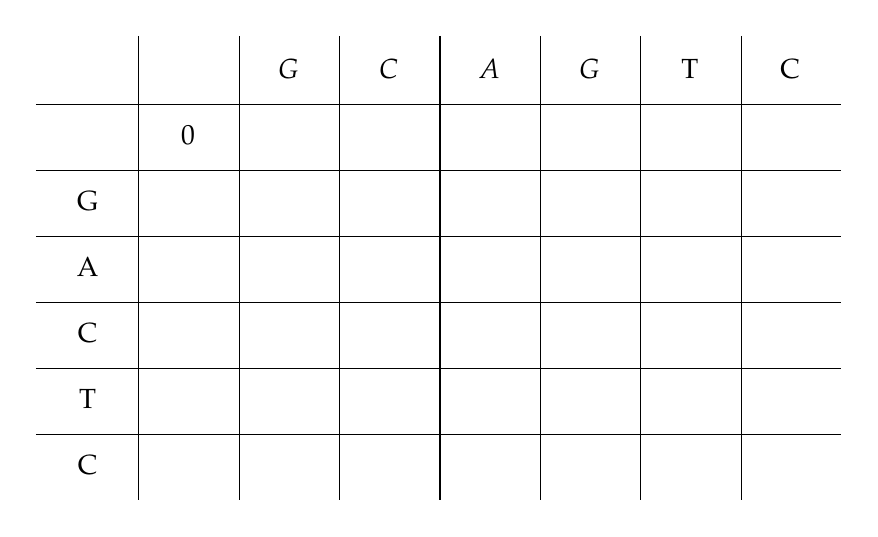
\begin{tikzpicture}
\matrix (mat) [table]
{
& & $G$ & $C$ & $A$ & $G$ & T & C \\
&0 &&&&&& \\
G & & & & & & &\\
A & & &  & & & &\\
C & & & & &  & &\\
T & & & & & &  &\\
C & & & & & & & \\
};
% the matrix rules
\foreach \x in {1,...,6}
{
  \draw 
    ([xshift=-.5\pgflinewidth]mat-\x-1.south west) --   
    ([xshift=-.5\pgflinewidth]mat-\x-8.south east);
  }
\foreach \x in {1,...,7}
{
  \draw 
    ([yshift=.5\pgflinewidth]mat-1-\x.north east) -- 
    ([yshift=.5\pgflinewidth]mat-7-\x.south east);
}    
% the arrows


\end{tikzpicture}


\noindent This is our score matrix with the base case that an empty alignment has a score of 0. \\ \\
\noindent
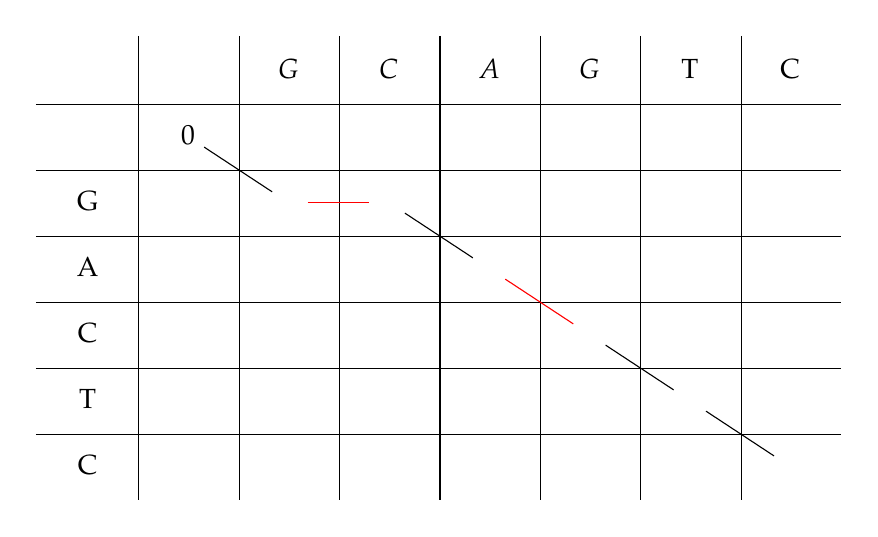
\begin{tikzpicture}
\matrix (mat) [table]
{
& & $G$ & $C$ & $A$ & $G$ & T & C \\
&0 &&&&&& \\
G & & & & & & &\\
A & & &  & & & &\\
C & & & & &  & &\\
T & & & & & &  &\\
C & & & & & & & \\
};
% the matrix rules
\foreach \x in {1,...,6}
{
  \draw 
    ([xshift=-.5\pgflinewidth]mat-\x-1.south west) --   
    ([xshift=-.5\pgflinewidth]mat-\x-8.south east);
  }
\foreach \x in {1,...,7}
{
  \draw 
    ([yshift=.5\pgflinewidth]mat-1-\x.north east) -- 
    ([yshift=.5\pgflinewidth]mat-7-\x.south east);
}    
% the arrows
\begin{scope}[shorten >=7pt,shorten <= 7pt]
\draw[-]  (mat-2-2.center) -- (mat-3-3.center);
\draw[red, -]  (mat-3-3.center) -- (mat-3-4.center);
\draw[-]  (mat-3-4.center) -- (mat-4-5.center);
\draw[red, -]  (mat-4-5.center) -- (mat-5-6.center);
\draw[-]  (mat-5-6.center) -- (mat-6-7.center);
\draw[-]  (mat-6-7.center) -- (mat-7-8.center);
\end{scope}

\end{tikzpicture}



\noindent
As you can see, a path through this matrix represents an alignment. Diagonal arrows represent matches or mismatchs while horizontal or vertical paths represent indels. The alignment represented by this path is \\
\texttt{G\textcolor{red}{C}A\textcolor{red}{G}TC} \\
\texttt{G\textcolor{red}{-}A\textcolor{red}{C}TC} \\ \\

\noindent Because horizontal and vertical paths represent indels, we can initialize the border from the base case as follows. \\
\noindent
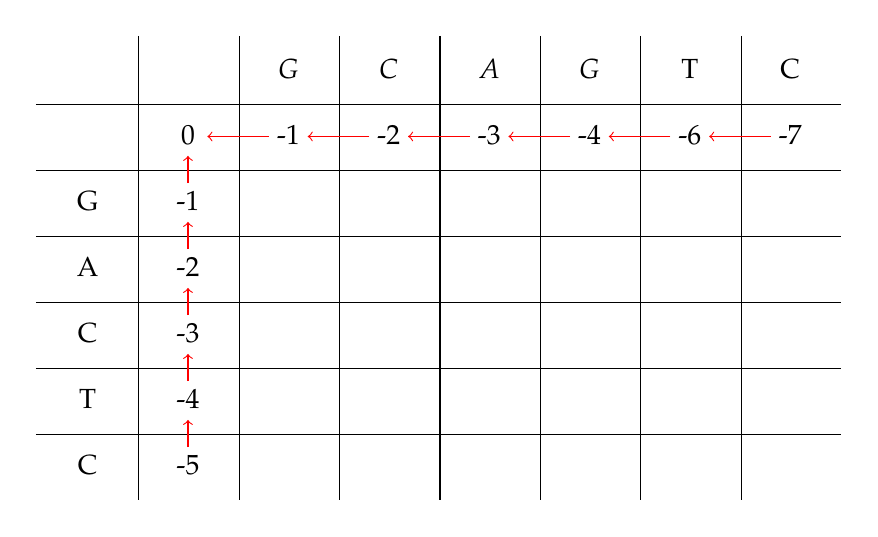
\begin{tikzpicture}
\matrix (mat) [table]
{
& & $G$ & $C$ & $A$ & $G$ & T & C \\
&0 &-1 &-2&-3&-4&-6&-7 \\
G & -1& & & & & &\\
A & -2& &  & & & &\\
C & -3 & & & &  & &\\
T & -4 & & & & &  &\\
C & -5 & & & & & & \\
};
% the matrix rules
\foreach \x in {1,...,6}
{
  \draw 
    ([xshift=-.5\pgflinewidth]mat-\x-1.south west) --   
    ([xshift=-.5\pgflinewidth]mat-\x-8.south east);
  }
\foreach \x in {1,...,7}
{
  \draw 
    ([yshift=.5\pgflinewidth]mat-1-\x.north east) -- 
    ([yshift=.5\pgflinewidth]mat-7-\x.south east);
}    
% the arrows
\begin{scope}[shorten >=7pt,shorten <= 7pt]
\draw[red,->]  (mat-2-3.center) -- (mat-2-2.center);
\draw[red,->]  (mat-2-4.center) -- (mat-2-3.center);
\draw[red,->]  (mat-2-5.center) -- (mat-2-4.center);
\draw[red,->]  (mat-2-6.center) -- (mat-2-5.center);
\draw[red,->]  (mat-2-7.center) -- (mat-2-6.center);
\draw[red,->]  (mat-2-8.center) -- (mat-2-7.center);
\draw[red,->]  (mat-3-2.center) -- (mat-2-2.center);
\draw[red,->]  (mat-4-2.center) -- (mat-3-2.center);
\draw[red,->]  (mat-5-2.center) -- (mat-4-2.center);
\draw[red,->]  (mat-6-2.center) -- (mat-5-2.center);
\draw[red,->]  (mat-7-2.center) -- (mat-6-2.center);
\end{scope}
\end{tikzpicture} \\ 

\noindent
We keep track of where we came from for each cell with a backtrace pointer. \\ \\
Now we fill out the score matrix with the following rules where $m$ is the scoring matrix and $s_1$ is the string/sequence 1 and $s_2$ is the string/sequence 2. \\

\begin{equation*}
m[i,j] = max
\begin{cases}
      m[i-1,j-1] + 1 & \text{if \,\, } s_1[i] = s_2[j] \text{ (match)} \\
      m[i-1,j-1] - 1 &  \text{if \,\, } s_1[i] \neq s_2[j] \text{ (mismatch)} \\
      m[i-1,j] - 1 \text{ (indel)} \\
      m[i,j-1] - 1 \text{ (indel)} \\
\end{cases}
\end{equation*}

\noindent
And keep an annotation of which cell we came from. Now we fill out all of the cells with these rules. Red arrows represent mismatches or indels. Dashed arrows represent equal scores which are ignored. If scores are equal, we favor matches or mismatches arbitrarily because we aren't looking for all optimal alignments, just one optimal alignment. \\ \\
\noindent
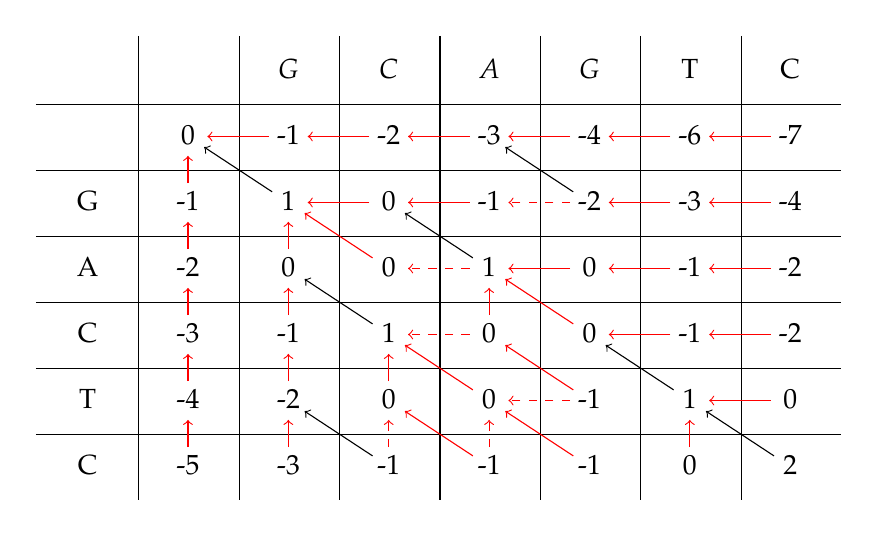
\begin{tikzpicture}
\matrix (mat) [table]
{
& & $G$ & $C$ & $A$ & $G$ & T & C \\
&0 &-1 &-2&-3&-4&-6&-7 \\
G & -1& 1 & 0 & -1 & -2 & -3 & -4 \\
A & -2& 0 & 0 & 1 & 0 & -1 & -2 \\
C & -3 & -1 & 1 & 0 & 0 & -1 & -2 \\
T & -4 & -2 & 0 & 0 & -1 &  1 & 0 \\
C & -5 &  -3 & -1 & -1 & -1 & 0 & 2 \\
};
% the matrix rules
\foreach \x in {1,...,6}
{
  \draw 
    ([xshift=-.5\pgflinewidth]mat-\x-1.south west) --   
    ([xshift=-.5\pgflinewidth]mat-\x-8.south east);
  }
\foreach \x in {1,...,7}
{
  \draw 
    ([yshift=.5\pgflinewidth]mat-1-\x.north east) -- 
    ([yshift=.5\pgflinewidth]mat-7-\x.south east);
}    
% the arrows
\begin{scope}[shorten >=7pt,shorten <= 7pt]
\draw[red,->]  (mat-2-3.center) -- (mat-2-2.center);
\draw[red,->]  (mat-2-4.center) -- (mat-2-3.center);
\draw[red,->]  (mat-2-5.center) -- (mat-2-4.center);
\draw[red,->]  (mat-2-6.center) -- (mat-2-5.center);
\draw[red,->]  (mat-2-7.center) -- (mat-2-6.center);
\draw[red,->]  (mat-2-8.center) -- (mat-2-7.center);
\draw[red,->]  (mat-3-2.center) -- (mat-2-2.center);
\draw[red,->]  (mat-4-2.center) -- (mat-3-2.center);
\draw[red,->]  (mat-5-2.center) -- (mat-4-2.center);
\draw[red,->]  (mat-6-2.center) -- (mat-5-2.center);
\draw[red,->]  (mat-7-2.center) -- (mat-6-2.center);
\draw[->]  (mat-3-3.center) -- (mat-2-2.center);
\draw[red,->]  (mat-3-4.center) -- (mat-3-3.center);
\draw[red,->]  (mat-3-5.center) -- (mat-3-4.center);
\draw[->]  (mat-3-6.center) -- (mat-2-5.center);
\draw[red,->]  (mat-3-7.center) -- (mat-3-6.center);
\draw[red,->]  (mat-3-8.center) -- (mat-3-7.center);
\draw[red,dashed,->]  (mat-3-6.center) -- (mat-3-5.center);
\draw[red,->]  (mat-4-3.center) -- (mat-3-3.center);
\draw[red,->]  (mat-4-4.center) -- (mat-3-3.center);
\draw[->]  (mat-4-5.center) -- (mat-3-4.center);
\draw[red,dashed,->]  (mat-4-5.center) -- (mat-4-4.center);
%\draw[red,->]  (mat-4-6.center) -- (mat-3-5.center);
\draw[red, ->]  (mat-4-6.center) -- (mat-4-5.center);
\draw[red,->]  (mat-4-7.center) -- (mat-4-6.center);
%\draw[red, ->]  (mat-4-7.center) -- (mat-3-6.center);
%\draw[red, ->]  (mat-4-8.center) -- (mat-3-7.center);
\draw[red, ->]  (mat-4-8.center) -- (mat-4-7.center);
\draw[red, ->]  (mat-5-3.center) -- (mat-4-3.center);
\draw[->]  (mat-5-4.center) -- (mat-4-3.center);
%\draw[red, ->]  (mat-5-5.center) -- (mat-4-4.center);
\draw[red, dashed, ->]  (mat-5-5.center) -- (mat-5-4.center);
\draw[red, ->]  (mat-5-5.center) -- (mat-4-5.center);
\draw[red, ->]  (mat-5-6.center) -- (mat-4-5.center);
\draw[red, ->]  (mat-5-7.center) -- (mat-5-6.center);
\draw[red, ->]  (mat-5-8.center) -- (mat-5-7.center);
\draw[red, ->]  (mat-6-3.center) -- (mat-5-3.center);
\draw[red, ->]  (mat-7-3.center) -- (mat-6-3.center);
\draw[red, ->]  (mat-6-4.center) -- (mat-5-4.center);
\draw[red, ->]  (mat-6-5.center) -- (mat-5-4.center);
\draw[red, ->]  (mat-6-6.center) -- (mat-5-5.center);
\draw[red, dashed, ->]  (mat-6-6.center) -- (mat-6-5.center);
\draw[ ->]  (mat-6-7.center) -- (mat-5-6.center);
\draw[red, ->]  (mat-6-8.center) -- (mat-6-7.center);
\draw[ ->]  (mat-7-4.center) -- (mat-6-3.center);
\draw[red, dashed, ->]  (mat-7-4.center) -- (mat-6-4.center);
\draw[red, ->]  (mat-7-5.center) -- (mat-6-4.center);
\draw[red, dashed, ->]  (mat-7-5.center) -- (mat-6-5.center);
\draw[red, ->]  (mat-7-6.center) -- (mat-6-5.center);
\draw[red, ->]  (mat-7-7.center) -- (mat-6-7.center);
\draw[ ->]  (mat-7-8.center) -- (mat-6-7.center);
\end{scope}
\end{tikzpicture} \\ 

\section*{Backtrace / Viterbi Algorithm}

Now to find the optimal global alignment, we start at the bottom righthand cell and follow our backtrace arrows to find the optimal path through the matrix. \\
\noindent
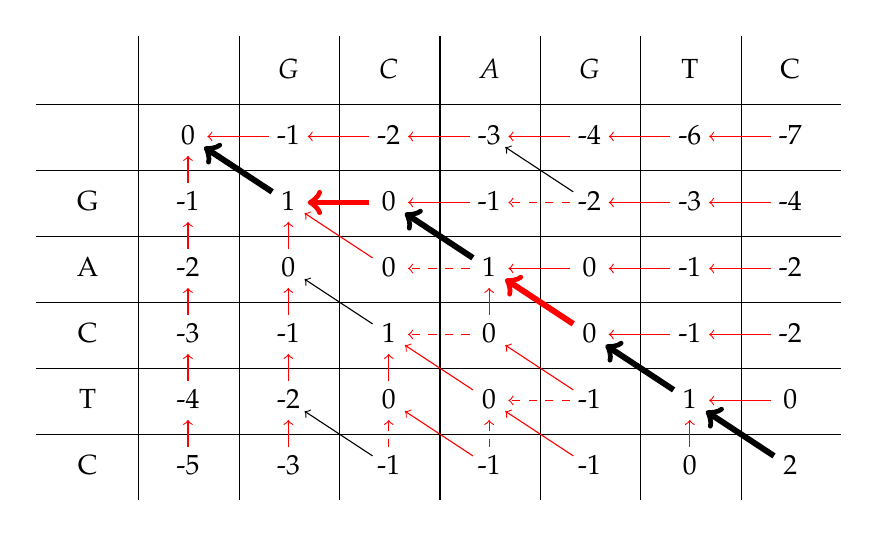
\begin{tikzpicture}
\matrix (mat) [table]
{
& & $G$ & $C$ & $A$ & $G$ & T & C \\
&0 &-1 &-2&-3&-4&-6&-7 \\
G & -1& 1 & 0 & -1 & -2 & -3 & -4 \\
A & -2& 0 & 0 & 1 & 0 & -1 & -2 \\
C & -3 & -1 & 1 & 0 & 0 & -1 & -2 \\
T & -4 & -2 & 0 & 0 & -1 &  1 & 0 \\
C & -5 &  -3 & -1 & -1 & -1 & 0 & 2 \\
};
% the matrix rules
\foreach \x in {1,...,6}
{
  \draw 
    ([xshift=-.5\pgflinewidth]mat-\x-1.south west) --   
    ([xshift=-.5\pgflinewidth]mat-\x-8.south east);
  }
\foreach \x in {1,...,7}
{
  \draw 
    ([yshift=.5\pgflinewidth]mat-1-\x.north east) -- 
    ([yshift=.5\pgflinewidth]mat-7-\x.south east);
}    
% the arrows
\begin{scope}[shorten >=7pt,shorten <= 7pt]
\draw[red,->]  (mat-2-3.center) -- (mat-2-2.center);
\draw[red,->]  (mat-2-4.center) -- (mat-2-3.center);
\draw[red,->]  (mat-2-5.center) -- (mat-2-4.center);
\draw[red,->]  (mat-2-6.center) -- (mat-2-5.center);
\draw[red,->]  (mat-2-7.center) -- (mat-2-6.center);
\draw[red,->]  (mat-2-8.center) -- (mat-2-7.center);
\draw[red,->]  (mat-3-2.center) -- (mat-2-2.center);
\draw[red,->]  (mat-4-2.center) -- (mat-3-2.center);
\draw[red,->]  (mat-5-2.center) -- (mat-4-2.center);
\draw[red,->]  (mat-6-2.center) -- (mat-5-2.center);
\draw[red,->]  (mat-7-2.center) -- (mat-6-2.center);
\draw[line width =.75mm, ->]  (mat-3-3.center) -- (mat-2-2.center);
\draw[line width = .75mm, red,->]  (mat-3-4.center) -- (mat-3-3.center);
\draw[red,->]  (mat-3-5.center) -- (mat-3-4.center);
\draw[->]  (mat-3-6.center) -- (mat-2-5.center);
\draw[red,->]  (mat-3-7.center) -- (mat-3-6.center);
\draw[red,->]  (mat-3-8.center) -- (mat-3-7.center);
\draw[red,dashed,->]  (mat-3-6.center) -- (mat-3-5.center);
\draw[red,->]  (mat-4-3.center) -- (mat-3-3.center);
\draw[red,->]  (mat-4-4.center) -- (mat-3-3.center);
\draw[line width = .75mm, ->]  (mat-4-5.center) -- (mat-3-4.center);
\draw[red,dashed,->]  (mat-4-5.center) -- (mat-4-4.center);
%\draw[red,->]  (mat-4-6.center) -- (mat-3-5.center);
\draw[red, ->]  (mat-4-6.center) -- (mat-4-5.center);
\draw[red,->]  (mat-4-7.center) -- (mat-4-6.center);
%\draw[red, ->]  (mat-4-7.center) -- (mat-3-6.center);
%\draw[red, ->]  (mat-4-8.center) -- (mat-3-7.center);
\draw[red, ->]  (mat-4-8.center) -- (mat-4-7.center);
\draw[red, ->]  (mat-5-3.center) -- (mat-4-3.center);
\draw[->]  (mat-5-4.center) -- (mat-4-3.center);
%\draw[red, ->]  (mat-5-5.center) -- (mat-4-4.center);
\draw[red, dashed, ->]  (mat-5-5.center) -- (mat-5-4.center);
\draw[red, ->]  (mat-5-5.center) -- (mat-4-5.center);
\draw[line width = .75mm, red, ->]  (mat-5-6.center) -- (mat-4-5.center);
\draw[red, ->]  (mat-5-7.center) -- (mat-5-6.center);
\draw[red, ->]  (mat-5-8.center) -- (mat-5-7.center);
\draw[red, ->]  (mat-6-3.center) -- (mat-5-3.center);
\draw[red, ->]  (mat-7-3.center) -- (mat-6-3.center);
\draw[red, ->]  (mat-6-4.center) -- (mat-5-4.center);
\draw[red, ->]  (mat-6-5.center) -- (mat-5-4.center);
\draw[red, ->]  (mat-6-6.center) -- (mat-5-5.center);
\draw[red, dashed, ->]  (mat-6-6.center) -- (mat-6-5.center);
\draw[line width=.75mm, ->]  (mat-6-7.center) -- (mat-5-6.center);
\draw[red, ->]  (mat-6-8.center) -- (mat-6-7.center);
\draw[ ->]  (mat-7-4.center) -- (mat-6-3.center);
\draw[red, dashed, ->]  (mat-7-4.center) -- (mat-6-4.center);
\draw[red, ->]  (mat-7-5.center) -- (mat-6-4.center);
\draw[red, dashed, ->]  (mat-7-5.center) -- (mat-6-5.center);
\draw[red, ->]  (mat-7-6.center) -- (mat-6-5.center);
\draw[red, ->]  (mat-7-7.center) -- (mat-6-7.center);
\draw[line width=0.75mm, ->]  (mat-7-8.center) -- (mat-6-7.center);
\end{scope}
\end{tikzpicture} \\ 

\noindent which creates the following alignment \\
\texttt{G\textcolor{red}{C}A\textcolor{red}{G}TC} \\
\texttt{G\textcolor{red}{-}A\textcolor{red}{C}TC} \\ \\



% Second Section %%%%%%%%%%%%%%%%%%%%%%%%%%%%%%%%%%%%%%%%%%%
% Fourth Section %%%%%%%%%%%%%%%%%%%%%%%%%%%%%%%%%%%%%%%%%%%
% Fifth Section %%%%%%%%%%%%%%%%%%%%%%%%%%%%%%%%%%%%%%%%%%%
% Add a figure %%%%%%%%%%%%%%%%%%%%%%%%%%%%%%%%%%%%%%%%%%%


% Fifth Section %%%%%%%%%%%%%%%%%%%%%%%%%%%%%%%%%%%%%%%%%%%
% Course Schedule %%%%%%%%%%%%%%%%%%%%%%%%%%%%%%%%%%%%%%%%%%%

\end{document}
